\documentclass[11pt,a4paper]{article}

% Page geometry
\usepackage[top=2.5cm, bottom=2.5cm, left=2.5cm, right=2.5cm]{geometry}

% Typography and encoding
\usepackage[T1]{fontenc}
\usepackage[utf8]{inputenc}
\usepackage{lmodern}
\usepackage{microtype}

% Mathematics
\usepackage{amsmath,amssymb,amsthm}

% Tables and arrays
\usepackage{booktabs}
\usepackage{tabularx}
\usepackage{array}
\usepackage{makecell}
\usepackage{multirow}

% Graphics and floats
\usepackage{graphicx}
\usepackage{float}
\usepackage{placeins}

% Utility packages
\usepackage{cite}
\usepackage{seqsplit}
\usepackage{url}
\usepackage{xcolor}
\usepackage{authblk}

% Additional formatting packages
\usepackage{caption}
\captionsetup[figure]{labelfont=bf,labelsep=space}
\captionsetup[table]{labelfont=bf,labelsep=space}
\usepackage{adjustbox}

% Hyperlinks
\usepackage[colorlinks=true,linkcolor=blue!75!black,citecolor=blue!75!black,urlcolor=blue!75!black]{hyperref}

% Title and authors
\title{\textbf{Exact Policy-Aware Regression Diagnosis for Precision-Constrained Threshold Selectors}}

% Authors
\author[1]{Thien Bao Nguyen\thanks{Corresponding author. Email: \texttt{baont@ueh.edu.vn}}}
\author[1]{Bao Tran Hoang\thanks{Email: \texttt{tranhoang.31251027696@st.ueh.edu.vn}}}
\author[1]{The Dang Khoa Tran\thanks{Email: \texttt{khoatran.31251020280@st.ueh.edu.vn}}}
\author[1]{Bao Han Nguyen\thanks{Email: \texttt{hannguyen.31251027458@st.ueh.edu.vn}}}
\author[1]{Trong Minh Nguyen\thanks{Email: \texttt{minhnguyen.31251023499@st.ueh.edu.vn}}}
\author[1]{Gia Han Tran\thanks{Email: \texttt{hantran.31251027103@st.ueh.edu.vn}}}
% Affiliation
\affil[1]{Institute of Intelligent and Interactive Technologies (3i Institute),
College of Technology and Design (CTD),
University of Economics Ho Chi Minh City (UEH),
Ho Chi Minh City, Vietnam}


\date{\today}

\emergencystretch=3em

\begin{document}

\maketitle

\begin{abstract}
Under the admitted finite-selector contract, regression tests at sampled precision targets cannot establish selected-ID equivalence throughout a continuous policy domain, potentially missing isolated differences at exact policy boundaries. Against configured variants proven divergent under the formal specification, a thirteen-point grid misses 26 of 183 variants (14.2\%) and a single-target snapshot misses 71 (38.8\%). In the executable program study, where an unchanged reference implementation provides an independent oracle, complete checking identifies all 136 nonconforming runs, whereas the grid identifies 111. On two documented upstream library defects in scikit-learn and SciPy, complete diagnosis matches grid detection on affected workloads while uniquely localizing exact boundary ownership and emitting independently checkable observation witnesses. The design has three layers: a formal diagnostic specification proving that continuous-domain equivalence reduces conditionally to finitely many exact checks; an input-bound diagnostic certificate with an independent streaming consumer; and empirical evaluations across 98 fixed-input comparison pairs, 360 mutant records, and the two historical upstream defects. Complete checking provides exact counterexample localization, boundary ownership, and certified reuse across query lattices, while streaming consumption eliminates full-mask materialization.
\end{abstract}

\vspace{0.5em}
\noindent\textbf{Keywords:} Software regression testing, Decision pipelines, Certifying computation, Precision constraints, Threshold selectors, Metamorphic testing.

\vspace{1em}

\section{Introduction}\label{sec:introduction}


\subsection{Background and Motivation}

Precision-constrained threshold selectors convert numerical scores into a set of observations for review or intervention. An alerting component in decision-support software (such as simulated pharmaceutical cold-chain temperature monitoring where excursions outside $[2^\circ\text{C}, 8^\circ\text{C}]$ require automated alerts) may support several precision targets as operating conditions change. A software modification must then be assessed against the permitted targets, rather than only the target selected for one regression test. This motivates the study; the evaluation assesses threshold selector components under stated contracts rather than an entire deployed enterprise system.

The relevant outcome is the selected set of observation IDs. Score differences alone do not determine whether that set changes, while agreement at one precision target does not establish agreement at other targets. Fixed labels and aligned IDs make this a finite empirical question: given two score/selector versions and a declared policy domain, where do selected memberships differ, who owns each boundary, and what evidence lets another implementation check the answer?

An existence test and a complete diagnosis answer different questions. A failing grid test supplies one observed difference. A complete diagnosis must also establish the scope outside that observation and retain isolated policy values. A singleton mismatch has zero interval length, so an interval-length summary cannot replace an equivalence verdict. Numerical interfaces create a further distinction: an exact decimal policy and the exact rational embedding of a binary64 value need not denote the same target.


\subsection{Research Gap and Related Work}

Constrained threshold selection and ranking have established foundations \cite{rath2022optimizing,mackey2018constrained,tasche2018plugin}, with documented calibration and public selector interfaces \cite{sklearn_calibrated,sklearn_tuned,behring2026evaltoolkit}. Regression verification \cite{godlin2009regression}, parameter synthesis \cite{storm2026parametric,junges2024parameter,dehnert2015prophesy}, predicate enumeration, SMT-based predicate abstraction and AllSMT \cite{mathsat_api,morettin2017efficient,spallitta2025disjoint} already provide ways to reason beyond sampled inputs. Certifying computations \cite{alkassar2013framework,mcconnell2011certifying} and proof-carrying approaches \cite{necula2002proof} establish the separation between producing a result and checking evidence. Metamorphic testing of classifiers and optimization software \cite{duquetorres2025assessing,yang2021towards,xie2011testing}, robust classification \cite{provost2001robust} and parametric monitoring \cite{chen2009parametric} address related testing or parameter-dependent questions.

While parameter synthesis and SMT-based predicate abstraction explore parameter regions in general formal verification, general-purpose solvers incur encoding and enumeration overheads whose performance depends heavily on formula structure (as demonstrated in our SMT AllSMT comparisons), and existing verification workflows do not provide a specialized, input-bound membership certificate format tailored for streaming regression pipelines. Conversely, traditional fixed-grid and single-target regression tests cannot guarantee detection of isolated boundary mismatches having zero Lebesgue measure (singleton mismatches) unless the relevant critical policies are explicitly included. A third potential alternative, \textit{boundary-aware direct probing}, exhaustively evaluates all critical policy thresholds but re-evaluates candidate sets repeatedly across probes, incurring candidate-scanning costs bounded by $\mathcal{O}((K+C)G)$ and leaving no persistent, independently verified proof artifact in the evaluated stateless baseline.

The question studied here is how those foundations can establish one specific observable under one explicit contract: selected-ID equality throughout a permitted precision domain, including endpoint ownership and the actual numerical policy interface. A complete-region answer is useful only if its cuts cover every admitted change, its memberships refer to the same observations, and its certificate can be checked against the original inputs. For executable adapters, those requirements must also delimit when collected guard events are sufficient and when the method must refuse certification.

The resulting contribution is an integrated diagnostic specification and its evaluated architecture. While the finite partitioning of feasibility regions under finite candidate sets is a natural structural reduction that builds upon predicate enumeration and interval analysis, this study's primary methodological novelty is the unified exact diagnostic framework: we formalize selected-ID equivalence over the continuous domain $[L, H]$ with exact observation-level counterexamples and Lebesgue PSC; we resolve exact boundary singletons and IEEE 754 floating-point preimage cuts; we devise an $\mathcal{O}(N \log N + G \log G + K)$ monotone heap sweep eliminating iterative solver overhead; and we encapsulate the result in an input-bound diagnostic certificate enabling independent streaming verification (verifiable against original inputs) with $\mathcal{O}(N+G+K+C)$ auxiliary storage and microsecond sub-domain query reuse.


\subsection{Research Objectives and Contributions}

This study investigates exact policy-aware regression diagnosis for precision-constrained threshold selectors. It integrates finite candidate-frontier analysis, complete policy-domain partitioning, selected-ID equivalence checking, exact boundary semantics, and input-bound diagnostic certificates within a unified verification workflow. The implementation further supports independently checked certificate consumption, rational and binary64 policy interfaces, and permitted-domain queries.

The evaluation combines fixed experimental cases, synthetic fixtures, fitted machine-learning pipelines, executable selector mutations, and documented upstream defect replays. The contributions are assessed against established verification and testing techniques rather than against earlier internal development versions of the same study.

Table~\ref{tab:1} summarizes the three research contributions alongside prior foundations and empirical evidence. Detailed formal proofs, extended benchmark factorials, defect replays, and reproducibility instructions are provided in the Supplementary Material (Online Resource~1, referenced throughout this paper by section numbers S1--S24 and tables S1--S17). Streaming consumption, the Boolean query index and CLI integration are supporting implementations. Their experiments assess engineering feasibility under the same diagnostic contract. The evaluation uses fixed observation arrays and recorded outcomes, with workload dependence and numerical assumptions made explicit.

\begin{table}[!htbp]
\caption{Contribution summary: foundational baselines, novel specifications, and empirical validation}\label{tab:1}
\centering
\footnotesize
\setlength{\tabcolsep}{3.5pt}
\renewcommand{\arraystretch}{1.2}
\begin{tabularx}{\textwidth}{@{} >{\raggedright\arraybackslash}p{2.2cm} >{\raggedright\arraybackslash}X >{\raggedright\arraybackslash}X >{\raggedright\arraybackslash}X @{}}
\toprule
\textbf{Layer} & \textbf{Foundational baseline} & \textbf{This study's specification} & \textbf{Empirical validation} \\
\midrule
\textbf{Formal} & Parameter synthesis and predicate enumeration \cite{storm2026parametric,mathsat_api} & Selected-ID equivalence over $[L, H]$; boundary singletons; IEEE 754 float preimages & Finite-partition reduction (Prop.~S1); exact certificate contract (Prop.~S5) \\
\midrule
\textbf{Evidential} & Certifying algorithms and producer/checker separation \cite{alkassar2013framework,mcconnell2011certifying} & Input-bound streaming consumer with SHA-256 digests; $\mathcal{O}(1)$ simultaneously active masks & 428 certificates replayed; $28.3\times$ memory reduction vs. materialized checker (Table~\ref{tab:9}) \\
\midrule
\textbf{Empirical} & Pointwise snapshots, 13-point grid, and direct boundary probing & Exact divergence localization, PSC metric, and $\mathcal{O}(\log(M+1))$ query reuse ($17\text{--}28\ \mu\text{s}$) & $183/183$ configured variants; $136/136$ executable nonconformances; $52.0\times$ measured sweep core speedup on Digits \\
\bottomrule
\end{tabularx}
\end{table}
\FloatBarrier


\subsection{Research Questions}

RQ1 --- Correctness: Does the implementation satisfy the finite contract's equivalence, coverage, endpoint and witness obligations on the evaluated inputs?

RQ2 --- Testing effectiveness and diagnosis: What do complete checking and point-based tests reveal on controlled variants and documented upstream defects, and what exact diagnostic information is added?

RQ3 --- Computational cost: What are the costs of constructing and independently checking complete diagnostics under matched output obligations?

RQ4 --- Policy-domain interpretation: How do declared policy sets and numerical-interface semantics change the diagnostic answer, and what costs accompany certificate reuse?


\section{Research Methodology}

The design has three layers. The formal diagnostic method defines the observable, completeness conditions and certificate obligations (\S\S\ref{subsec:problem}--\ref{subsec:cert}). Empirical validity studies challenge those conditions with fixed-input comparisons, executable changes, numerical interfaces and documented defects (\S\ref{subsec:boundary}). Engineering feasibility studies measure production, checking and query costs under separately specified protocols (\S2.5). Fig.~\ref{fig:1} shows the common workflow; optimizations operate within it. Authoring scripts, baseline adapters and execution harnesses were developed with assistance from generative AI tools (OpenAI Codex), with human verification of all code, outputs and formal arguments.

\begin{figure}[!htbp]
\centering

\includegraphics[height=0.5\textheight]{figures/fig1.png}
\caption{Diagnostic workflow under the admitted finite contract. A complete input-bound certificate separates producer and independent streaming consumer}\label{fig:1}
\end{figure}
\FloatBarrier


\subsection{Problem Formulation and Selector Contract}\label{subsec:problem}

Observation IDs are unique and aligned across versions; labels are binary and fixed, and scores are finite. Each version s has a finite family of nonempty threshold candidates. A candidate contains a complete score-tie group prefix, with actual positive count k and selected size n. Inclusive feasibility compares its exact empirical precision k/n with policy $\alpha$. Among feasible candidates the reference selector maximizes actual positive count, then selected size; it abstains if none is feasible or all labels are negative. The following expression uses a version index consistently for the maximizer and selected set:
\begin{equation}
j_{s}^{*}(\alpha) = \arg\max_{j:\; \alpha n_{s,j} \le k_{s,j}} (k_{s,j}, n_{s,j}), \quad S_{s}(\alpha) = C_{s,j_{s}^{*}(\alpha)} \label{eq:selector}
\end{equation}
If the feasible candidate set is empty, or all observation labels are negative, $S_s(\alpha) = \varnothing$ by definition; the $\arg\max$ expression applies only when a feasible non-abstaining candidate exists.

The permitted domain $\mathcal{A} = [L, H]$ has exact rational endpoints with $0 \le L < H \le 1$. $\alpha = 0$ follows the same feasibility and abstention rules. Alternative candidate families, fixed priorities and strict-feasibility contracts are represented explicitly in the controlled studies; they do not silently change the reference objective. The output is a Boolean equivalence verdict, complete divergent cells with boundary closure, and an observation witness for each distinct divergent state:
\begin{equation}
\mathcal{D}_{\mathcal{A}} = \{\alpha \in [L, H] : S_{\mathrm{old}}(\alpha) \neq S_{\mathrm{new}}(\alpha)\}, \quad \mathrm{PSC} = \frac{\mathrm{length}(\mathcal{D}_{\mathcal{A}})}{H - L} \label{eq:psc}
\end{equation}

PSC is the exact divergent interval-length fraction. It is neither a deployment probability nor a substitute for the Boolean verdict: an affected singleton contributes zero length. Selected counts also do not generally establish selected-ID equality, because score order may change between versions. The method therefore checks memberships under aligned identities.


\subsection{Exact Policy-Domain Verification}\label{subsec:spec}

Completeness requires a fixed finite candidate family, policy-independent candidate memberships and priorities, and a complete representation of every feasibility-guard change. For exact rational guards, the critical set B contains L, H and every candidate feasibility ratio of either version strictly inside A. These conditions are assumptions of the theorem, not consequences of observing a few executable traces.

Finite partition theorem. Under those conditions, both selected memberships are constant on every open interval between consecutive values of B. Equality throughout A holds if and only if memberships agree at every singleton B value and one representative in each nonempty open interval.

Proof. No admitted feasibility predicate changes inside an open interval without crossing its fixed ratio. Fixed memberships, priorities and abstention then keep the selected set constant. Singletons and open intervals partition the domain, giving necessity and sufficiency. Singleton tests retain inclusive/strict boundary behavior; midpoint testing is sufficient only after the complete critical set is established. Table~\ref{tab:2} separates mathematically sufficient conditions, implementation-enforced checks and trusted assumptions.

\begin{table}[!htbp]
\caption{Assurance boundary: mathematically sufficient conditions, implementation-enforced checks and trusted assumptions}\label{tab:2}
\centering
\footnotesize
\setlength{\tabcolsep}{3.5pt}
\renewcommand{\arraystretch}{1.15}
\begin{tabularx}{\textwidth}{@{} >{\raggedright\arraybackslash}p{2.8cm} >{\raggedright\arraybackslash}X >{\raggedright\arraybackslash}p{3.2cm} @{}}
\toprule
\textbf{Assurance layer} & \textbf{Description} & \textbf{Where established} \\
\midrule
Mathematically sufficient conditions & Finite candidate family with fixed priority and policy-independent membership; exact endpoint ownership; finite-partition theorem (Prop. S1); membership certificate obligations (Prop. S5) & Main \S\ref{subsec:spec}; Online Resource~1 (Sections~S1.1--S1.3) \\
\midrule
Implementation-enforced checks & SHA-256 input digest binding; ordered coverage and unique endpoint ownership validated by independent consumer; AST guard-placement check for source adapters; runtime refusal on unsupported fixtures & Main \S\ref{subsec:cert}; Online Resource~1 (Sections~S3--S4 and S17) \\
\midrule
Trusted assumptions (not machine-checked) & Python/NumPy/SciPy score computation faithfully represents intended arithmetic; source adapter corpus covers only guarded $\alpha$ arguments; observer instrumentation does not change program semantics & Main \S\ref{subsec:cert}; Online Resource~1 (Sections~S1.6 and S3) \\
\bottomrule
\end{tabularx}
\end{table}
\FloatBarrier

For a public binary64 policy interface, a guard can change at a rounding preimage rather than at the displayed rational precision. The floating-point preimage perspective follows established numerical reasoning \cite{andrlon2023finding}. Under IEEE 754 standard roundTiesToEven semantics \cite{ieee2019floating}, if p is an observed finite binary64 precision and q is its next larger representable value, nearest-even conversion changes side at the exact rational midpoint c=(p+q)/2; equality at c belongs to the even significand, with guard-specific midpoint ownership established in Lemma S6. The admitted model uses the union of those guard cuts, rational-reference ratios and domain endpoints, with explicit ownership. It requires the stated conversion mode and policy-independent candidates and priorities. Additional state or unrepresented policy-dependent branches invalidate the coverage argument.

The implementation sorts scores, forms exact TP/N ratios and sweeps the critical policies. Fixed-priority candidates are discarded when they become infeasible. For equal-sized score prefixes, inverse ranks and prefix maxima test selected-ID equality in constant time after preprocessing; distinct divergent state pairs are scanned for changed-row counts and an ID witness. Adjacent identical states are merged only while preserving boundary closure. For N rows, G total candidates, K critical values and D distinct divergent state pairs, core work is $\mathcal{O}(N \log N + G \log G + K)$, with $\mathcal{O}(ND)$ witness work and O(N+G+K) auxiliary storage under unit-cost rational operations. Arbitrary-precision operand costs, hashing and serialization are additional. Complete proofs and their assumptions are in Online Resource~1 (Section~S1). Table~\ref{tab:3} summarizes the algorithmic time and space complexity across the four diagnostic components.

\begin{table}[!htbp]
\caption{Principal asymptotic complexity for the four diagnostic components (dominant terms; see Section~S1 for full technical bounds including tie-sorting and probe-ordering terms; $N$ observations, $G$ threshold candidates, $C$ certificate cells, $K$ critical values, $D$ distinct divergent pairs, $M$ maximal divergent components)}\label{tab:3}
\centering
\footnotesize
\setlength{\tabcolsep}{3pt}
\renewcommand{\arraystretch}{1.2}
\begin{tabularx}{\textwidth}{@{} >{\raggedright\arraybackslash}p{2.4cm} >{\raggedright\arraybackslash}p{3.4cm} >{\raggedright\arraybackslash}p{2.1cm} >{\raggedright\arraybackslash}X @{}}
\toprule
\textbf{Component} & \textbf{Principal time} & \textbf{Space complexity} & \textbf{Operational characteristics} \\
\midrule
\textbf{Producer} (exact sweep) & $\mathcal{O}(N \log N + G \log G + K + ND)$ & $\mathcal{O}(N + G + K + C)$ & Monotone heap sweep across $K$ critical atoms; extracts witnesses for $D$ distinct divergent pairs; unit rational ops (Prop.~S3). \\
\midrule
\textbf{Materialized checker} (unstreamed) & $\mathcal{O}(NG + (K + C)G + NC)$ & $\mathcal{O}(NG + C)$ & Materializes and retains all $G$ candidate threshold masks in memory ($\mathcal{O}(NG)$ space); scans candidates at all $2K-1$ probes. \\
\midrule
\textbf{Streaming checker} (consumer) & $\mathcal{O}(NG + (K + C) \log G + ND)$ & $\mathcal{O}(N + G + K + C)$ & Streams one mask at a time ($\mathcal{O}(1)$ active masks); bisection on suffix winners; verifies digest and witnesses (Prop.~S5). \\
\midrule
\textbf{Query index} (Boolean lattice) & $\mathcal{O}(C \log C)\text{ build}$; $\mathcal{O}(\log(M + 1))\text{ query}$ & $\mathcal{O}(M + 1)$ & Post-verification index over $M$ maximal divergent components; sub-domain interval/point queries in $\approx 17\text{--}28\ \mu\text{s}$ ($\mathcal{O}(1)$ if $M=0$). \\
\bottomrule
\end{tabularx}
\end{table}
\FloatBarrier


\subsection{Independent Certificate Checking and Executable Admission}\label{subsec:cert}

A certificate binds the inputs by SHA-256 and records selector contracts, domain, critical fractions, cells, membership counts, equivalence, witnesses and PSC. The independent consumer reconstructs threshold masks from the original arrays, derives its own critical values and verifies coverage, unique endpoint ownership, winners, actual memberships, witnesses and changed-row counts. It recomputes the verdict and divergent length. Agreement of counts alone is insufficient, and checking one witness alone does not verify an entire negative region.

The certificate is an independently consumable diagnostic object, not a machine-checked proof of arbitrary Python behavior. Producer and consumer have separate implementations but share the mathematical contract and numerical dependencies. The streaming consumer reduces retained mask materialization without removing worst-case $\mathcal{O}(NG)$ counting/reconstruction work; its detailed suffix reasoning, operand costs and additional sorting terms are in Online Resource~1 (Section~S1). The Boolean index changes query output work after a full certificate check and remains a supporting engineering component.

Executable-source evaluation uses an unchanged direct-mask reference, actual selected-ID outputs and an explicit admission boundary. The tested programs restrict policy dependence to the instrumented guard, keep candidates and priorities independent of policy, and retain source/input bindings and repeated guard-event consistency checks. AST checks and sampled traces alone do not establish these properties for arbitrary Python. Unreviewed sources, hidden state, unsupported policy dependence and invalid outputs are refused rather than certified. Public-library adapters instead declare their own finite-candidate and numerical-interface contracts. Online Resource~1 (Sections~S3, S4, and S5) document those distinct boundaries.

To make the assurance structure explicit and avoid conflating different validation regimes, Table~\ref{tab:assurance_taxonomy} categorizes the assurance boundaries across the five evaluation cohorts, delineating the oracle source, independent checking mechanism, and admissible scientific conclusion for each study.

\begin{table}[!htbp]
\caption{Assurance taxonomy across evaluation cohorts: oracle provenance, independent verification mechanisms, and admissible empirical conclusions}\label{tab:assurance_taxonomy}
\centering
\footnotesize
\setlength{\tabcolsep}{3pt}
\renewcommand{\arraystretch}{1.15}
\begin{tabularx}{\textwidth}{@{} >{\raggedright\arraybackslash}p{2.3cm} >{\raggedright\arraybackslash}p{2.6cm} >{\raggedright\arraybackslash}X >{\raggedright\arraybackslash}X @{}}
\toprule
\textbf{Study cohort} & \textbf{Oracle provenance} & \textbf{Independent checking mechanism} & \textbf{Admissible conclusion} \\
\midrule
Declared-semantics mutants (183 variants) & Pure mathematical specification (exact precision, lexicographic $(k, n)$ order) & Separately implemented streaming consumer re-evaluating raw arrays; SHA-256 digest validation & Complete divergence localization on declared candidate models; exposes point-grid blindspots. \\
\midrule
Executable SUT conformance (136 nonconforming) & Unchanged reference Python module + AST guard audit & Runtime execution trace replay; bitset comparison of observed IDs vs. reference output & Dynamic program conformance under audited policy-guard assumption; safe refusal on unsupported code. \\
\midrule
Public library APIs (scikit-learn \& eval-toolkit) & Documented public interfaces with custom scorer & Cross-comparison of public API outputs against exact rational certificate & API integration feasibility without internal tampering; zero regressions on supported configs. \\
\midrule
Upstream defect replays (scikit-learn \& SciPy) & Official upstream bug fixes and maintainer release commits & Differential replay between affected and fixed versions on frozen workloads & Real-world diagnostic scope, boundary ownership, and ID localization; not novel bug discovery. \\
\midrule
Numerical interface (Binary64 vs. Rational) & IEEE 754 roundTiesToEven arithmetic & Preimage boundary enumeration and exact rational cut validation & Semantic divergence risk between decimal targets and binary64 floats; no defect attribution. \\
\bottomrule
\end{tabularx}
\end{table}
\FloatBarrier


\subsection{Empirical Validity Design and Condition Coverage}\label{subsec:boundary}

The evaluation uses 98 fixed input pairs assembled during the development of this study, comprising 50 retained experimental comparisons, 17 synthetic fixtures, one public WDBC pilot, and 30 newly fitted pipeline inputs. The retained cases and synthetic fixtures were constructed and preserved during earlier development stages of the same research project; they do not originate from a separate prior publication. The original input files and experimental records are maintained to support reproducibility. The 30 pipeline inputs use ten seeded splits from each of WDBC logistic/isotonic, digits zero-vs-rest LinearSVC/sigmoid and generated imbalanced random-forest/quantized-score families. Fitting, calibration and evaluation indices are disjoint and recorded; RF reserves its unused calibration split. Evaluation labels define the empirical selector, not a deployable test-label-free prediction rule. The 255 stored grid configurations are cross-checked against their bundled CSV records. The 50 comparison pairs and their 255 grid configurations are constructed from a simulated pharmaceutical cold-chain temperature telemetry monitoring scenario ($N=37{,}471$ observations, $G=87$ candidate thresholds), where ground-truth alert labels are determined by deterministic rule-based domain criteria adhering to standard pharmaceutical cold-chain specifications: sensor readings within the $[2^\circ\text{C}, 8^\circ\text{C}]$ range denote compliant holding conditions ($y_i=0$), whereas excursion readings outside $[2, 8]^\circ\text{C}$ trigger alerts ($y_i=1$). The 17 synthetic fixtures provide controlled edge cases targeting boundary clustering, tie saturation, and extremal feasibility. This evaluation suite was directly developed and structured within this research project to stress-test policy-domain regression diagnosis across varying candidate densities and tie structures.

The conditions target different assumptions rather than represent independent deployments (Table~\ref{tab:4}). The 30 pipeline inputs range from 143 to 600 rows and from 4 to 450 distinct score candidates; the fraction of observations in non-singleton score groups spans 0 to 1. These ranges are descriptive checks of the frozen arrays. Tie/candidate stress, identity violations, boundary changes and numerical conversion have different diagnostic roles; they are not pooled into one diversity score.

\begin{table}[!htbp]
\caption{Recorded condition coverage and its diagnostic purpose. Ranges describe frozen arrays; conditions are not independent deployments or a fully crossed industrial sample}\label{tab:4}
\centering
\footnotesize
\setlength{\tabcolsep}{3.5pt}
\renewcommand{\arraystretch}{1.15}
\begin{tabularx}{\textwidth}{@{} >{\raggedright\arraybackslash}p{2.8cm} >{\raggedright\arraybackslash}X >{\raggedright\arraybackslash}X @{}}
\toprule
\textbf{Condition} & \textbf{Recorded variation} & \textbf{Diagnostic obligation challenged} \\
\midrule
Ties and candidate counts & 30 pipeline inputs: N 143--600, G 4--450; tied-observation fraction 0--1. Designed G 10/30/90/250/500. & Complete tie groups, candidate selection and count-dependent work \\
Score structure and identities & Quantization, roundoff tie splitting, within-tie prefixes; 30 ID violations and aligned-permutation controls & Membership equality beyond score/count agreement; aligned identities \\
Guard and priority semantics & Inclusive/strict precision, threshold comparison, omitted candidates, reversed secondary priority and feasibility counts & Fixed contract, complete policy cuts and correct winning membership \\
Numerical representation & Controlled float32 score casts; exact rational and binary64 policy interfaces; integer-axis defect fixtures & Exact conversion cuts and endpoint ownership, with distinct query embeddings \\
Boundaries and negative controls & Singleton/open-cell probes, PSC=0 mismatches; 57 equivalent fault variants and 90 valid controls & Boolean verdict separate from interval length; scoped false alarms \\
Unsupported execution & Twelve unsupported-source fixtures and three invalid-runtime-output fixtures & Refusal rather than an unsupported completeness claim \\
\bottomrule
\end{tabularx}
\end{table}
\FloatBarrier

For each fitted base input, eight selector/numerical variants, one row-ID fault and three valid controls yield 360 records. The separate program-conformance study executes a reference and six local changed programs on the same 30 inputs. Configured-contract divergence, actual executable nonconformance and input-identity violations retain separate denominators. Fault models include feasibility, threshold comparison, candidate omission, within-tie splitting, secondary priority, counting and numerical perturbation; Online Resource~1 (Sections~S3 and S6) retain operator-level details. Exhaustive tests cover 10{,}854 small score/label combinations, plus 1{,}000 seeded randomized cases and targeted endpoint, identity, abstention and tamper checks.

Two documented defects provide historical-source evidence: scikit-learn precision-recall truncation \#23213/\#23214 \cite{sklearn_issue23213,sklearn_pr23214} and SciPy nearest-interpolation integer overflow \#6318/\#6351 \cite{scipy_issue6318,scipy_pr6351}. Unchanged affected/fixed source bodies are executed through recorded compatibility bridges. The first study uses the report protocol and 30 pipeline workloads; the second uses six prespecified axes plus 30 constructed pipeline propagation fixtures. Their workloads are not independent defects or historical binary installations. SciPy release records provide dependency context \cite{scipy_news}. The installed eval-toolkit 1.12.0 public selector \cite{behring2026evaltoolkit} is a numerical-contract study, not a third confirmed defect; the installed TunedThresholdClassifierCV study \cite{sklearn_tuned} is another component of scikit-learn. Full contracts, source hashes and replay details are retained in Online Resource~1 (Sections~S2, S5, S7, and S8).


\subsection{Engineering Feasibility and Experimental Protocols}\label{subsec:feasibility}

Snapshot, grid, and boundary-aware direct probing baselines compare actual selected IDs under the same declared task. Snapshot uses $\alpha=0.50$; grid uses thirteen exact rational targets from 0.30 to 0.90. To directly assess whether the certificate-based framework provides empirical speedup and utility over simple exhaustive testing, we introduce a \textit{boundary-aware direct probing baseline}. This baseline derives the exact critical set $B = \{L, H\} \cup \{k/n \in (L, H)\}$ (with $K = |B|$ critical values including endpoints $L$ and $H$) and intermediate open-atom midpoints, evaluating both selector versions across all $2K-1$ canonical probe points (comprising $K$ boundary singletons and $K-1$ open-cell midpoints). We evaluate this baseline across two complementary perspectives: first, an empirically measured core comparison that evaluates identical preprocessed candidate descriptors across all $2K-1$ critical policy atoms to isolate core sweep speedups; and second, an analytical lifecycle decomposition that evaluates a hypothetical matched certification workflow under assumed shared packaging and streaming verification overheads to assess end-to-end cost tradeoffs. B4/current score guards observe score arrays and have a different scope from changed-selector execution. For complete-region costs, a direct Z3 encoding \cite{demoura2008z3} must return the same maximal divergent components, endpoint ownership, PSC, verdict and rational policy/row witnesses as the partition method. Residual UNSAT is required after cell enumeration; timeout or unknown prevents certification. This is a specified solver encoding, not a benchmark of an independently optimized AllSMT tool \cite{mathsat_api,spallitta2025disjoint}.

Each timing claim belongs to its protocol. Traced certificate production includes validation, construction, input hashing and JSON serialization, with ten repetitions per condition on one recorded Windows/Python 3.12.10 host; inputs precede tracing and peak auxiliary MiB excludes process RSS. Preparation-matched timings and untraced ablation remain separate. Complete-region factorials cross N={1{,}000,10{,}000,100{,}000}, G={10,30,90} and three candidate-omission patterns, retaining all 27 tasks with five randomized repetitions; six larger-candidate tasks use N=10{,}000, G={250,500} and three repetitions. Totals include preparation, production/serialization and the same independent region checker. Paired consumers use identical prepared certificates, five untraced repetitions and separate memory runs. Full phase definitions and chronological records are in Online Resource~1 (Sections~S9--S10 and S16).

Allowed-domain queries evaluate finite sets, exact decimal lattices and intervals with endpoint ownership. Representable binary64 probes are embedded by exact integer ratios and are kept separate from rational decimal targets. On 36 SciPy fixtures, eight prespecified scenarios are compared with direct masks and an independent selected-bitset Z3 encoding; witnesses are checked and unknown aborts the comparison. Reuse studies separate two certificate APIs, which both construct and independently check a complete record, from direct masks and incremental Z3, which answer the query without exporting/checking that complete record. Setup, checking, query and total costs remain separate. Online Resource~1 (Sections~S13--S15) contains the request plans, repetitions and unequal assurance obligations.


\section{Results}


\subsection{RQ1 Correctness and Exact Policy Equivalence}\label{subsec:rq1}

The recorded exact-archive execution reports 42 passing core tests (documented in detached evidence logs \texttt{stage\_logs/\allowbreak run\_all\_pytest.log} and \texttt{results/\allowbreak pytest.xml}) and 18 passing upstream threshold tests in separate suites. The independent consumers accept all 428 application/mutation certificates across 98 bound inputs and 41{,}348 policy probes, checking coverage, memberships, endpoints and witnesses. Altered bindings, partitions, winners and metrics are rejected in targeted tests. These results support the implemented finite obligations on the evaluated inputs, while the proof supplies their conditional rationale. Execution logs and the historical distinction from earlier internal development snapshot files (\texttt{artifact\_verification.json} with 41 tests) are mapped in Online Resource~1 (Section~S21).

Policy sensitivity varies across the four fixed-input cohorts (Table~\ref{tab:5}). All 255 stored grid outcomes and their selected counts match the complete record. Within the 23 cases represented by those grid records, the same 15 cases are sensitive under both procedures; complete checking provides their regions. For the public WDBC pilot, the divergent set is exactly (43/51,9/10] on $[3/10, 9/10]$, with excluded left boundary, length 29/510 and PSC=29/306. The grid's affected values 0.85 and 0.90 lie inside that set. Among 30 float32-cast pipeline comparisons, only digits\_svc\_sigmoid\_seed2 is policy-sensitive, with PSC=25/5084.

\begin{table}[!htbp]
\caption{Fixed-input cohorts and policy-sensitive comparisons under their declared domains}\label{tab:5}
\centering
\footnotesize
\setlength{\tabcolsep}{3.5pt}
\renewcommand{\arraystretch}{1.15}
\begin{tabularx}{\textwidth}{@{} >{\raggedright\arraybackslash}X c c >{\raggedright\arraybackslash}p{3.2cm} @{}}
\toprule
\textbf{Cohort} & \textbf{Pairs} & \textbf{Policy-sensitive pairs} & \textbf{Domain} \\
\midrule
Independent\_pipeline & 30 & 1 & $[0.30, 0.90]$ \\
Public\_WDBC & 1 & 1 & $[0.30, 0.90]$ \\
Retained & 50 & 40 & [0.30,0.80] \\
Synthetic & 17 & 11 & [0.30,0.80] \\
\bottomrule
\end{tabularx}
\end{table}
\FloatBarrier

The endpoint-only example in \S\ref{subsec:rq2} shows why the successful membership/coverage checks must retain the Boolean verdict separately from PSC. Neither the observed sensitive-case fraction nor certificate acceptance estimates a population defect rate or proves unrestricted program correctness.


\subsection{RQ2 Testing Effectiveness and Diagnostic Information}\label{subsec:rq2}

The 183 divergent variants are those established by independently checked certificates; grid13 misses 26 (14.2\%) and snapshot misses 71 (38.8\%). In the executable study, where the unchanged reference program provides an independent oracle, complete checking identifies all 136 nonconforming runs and the grid 111 (Fig.~\ref{fig:2}). Of the 26 grid misses on configured variants, 15 have positive-length divergent regions and 11 differ only at singletons.

\begin{figure}[!htbp]
\centering
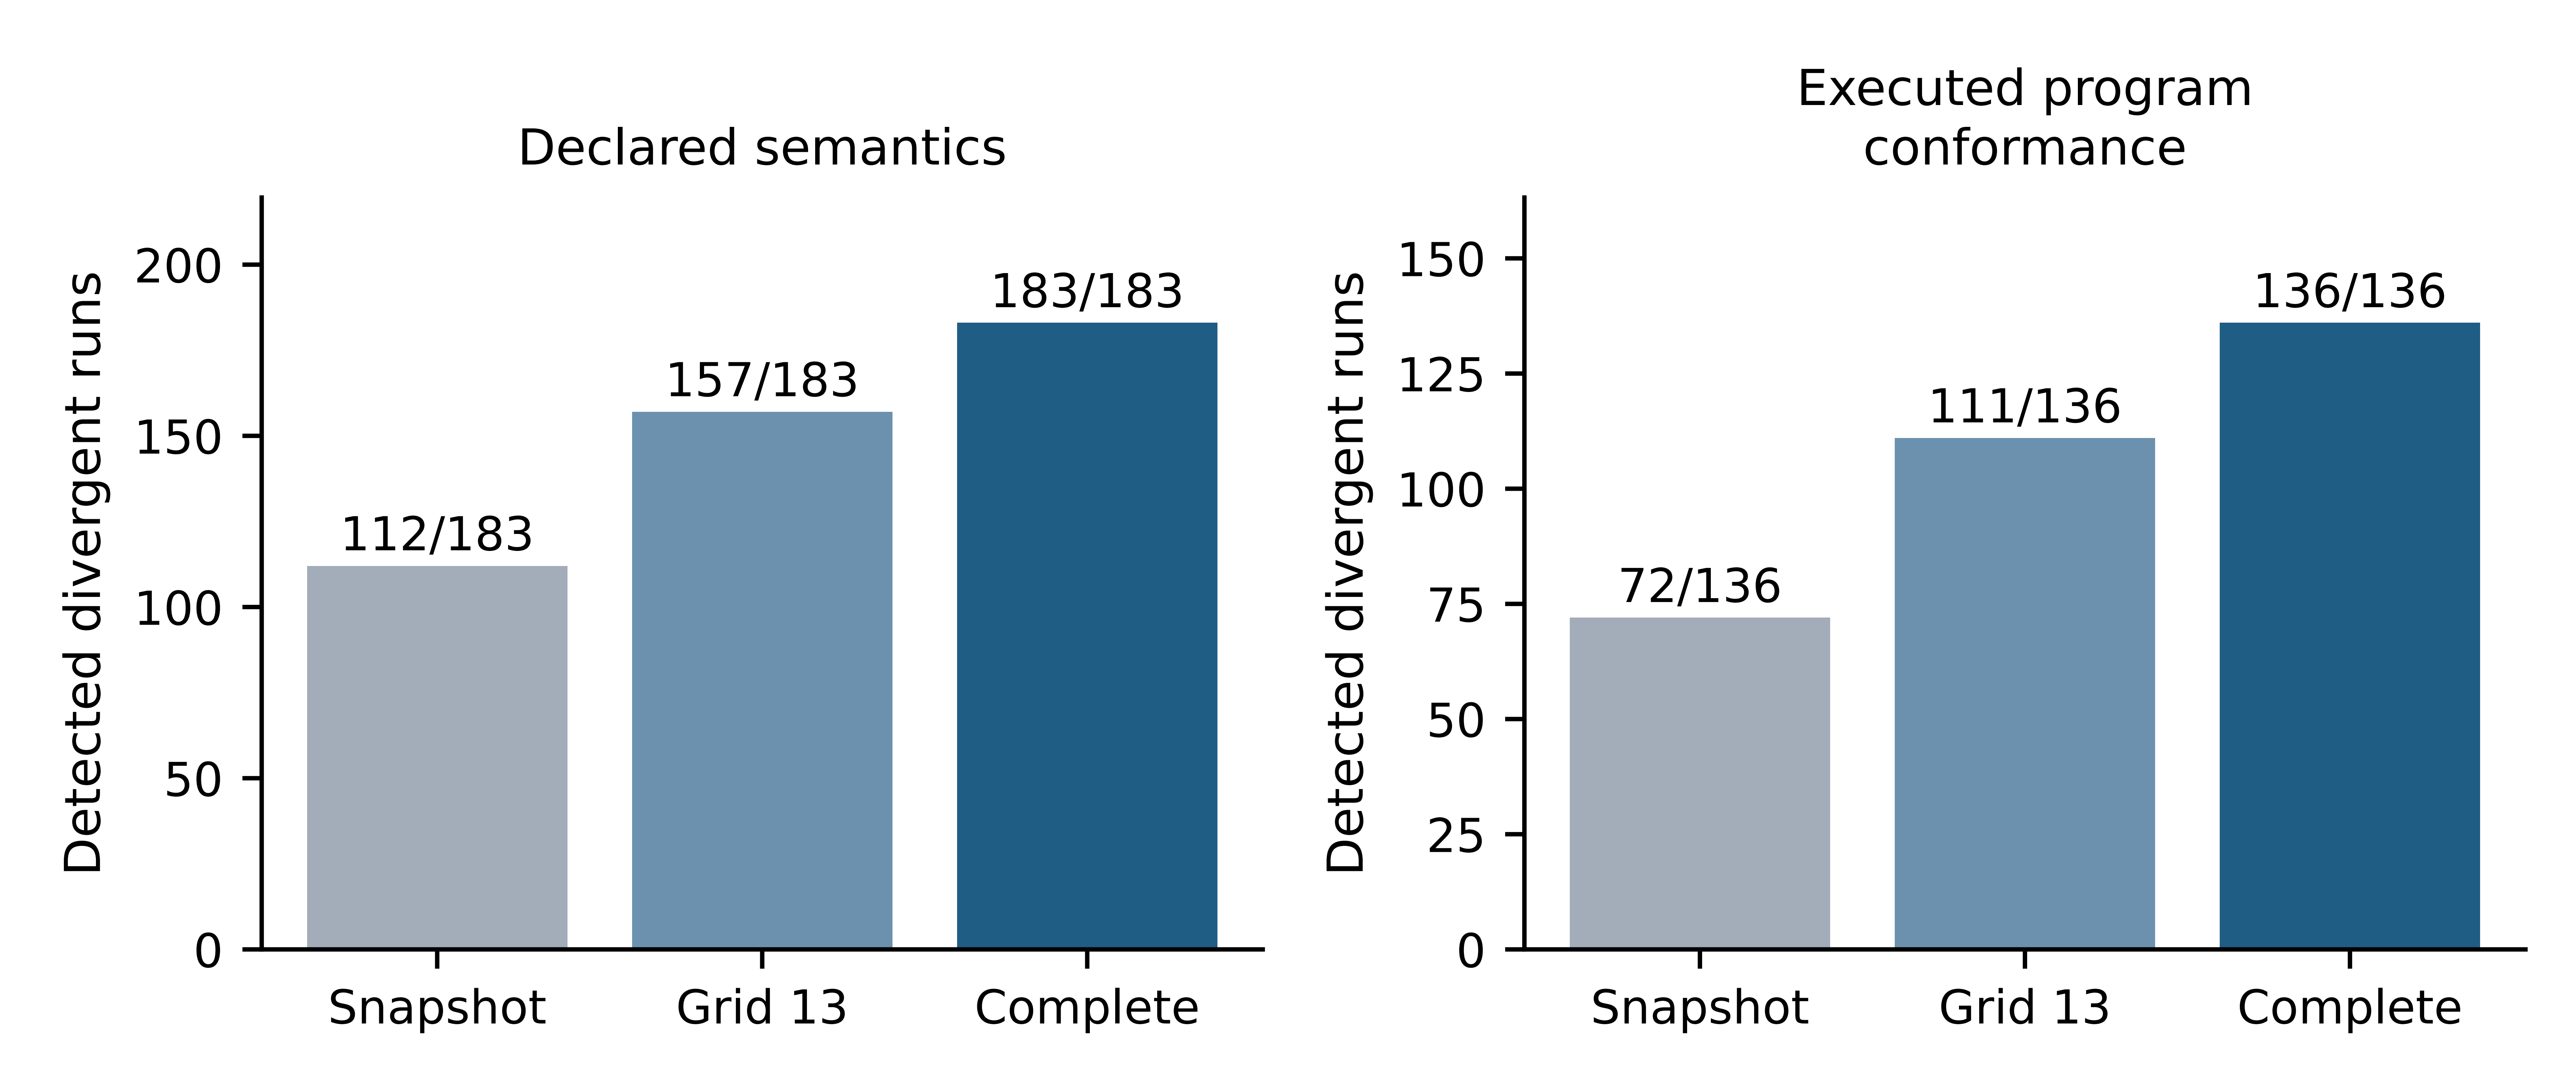
\includegraphics[width=0.88\textwidth]{figures/fig2.png}
\caption{Detection under two distinct evaluation contracts. Configured divergence and executed nonconformance denominators are not pooled}\label{fig:2}
\end{figure}
\FloatBarrier

Table~\ref{tab:6} retains the declared-contract baseline observations. Among the 360 total records, 57 fault variants are equivalent on the tested input/domain, 30 row-ID violations are rejected separately, and no exact policy alarm occurs on the 90 valid controls. B4 and the current guard raise 9 and 42 structural flags on observed policy-equivalent variant/control runs. Their different observable prevents interpreting every flag as a policy error or every missed selector change as a failure of their original score-structure task.

\begin{table}[!htbp]
\caption{Detection under declared selector semantics; the denominator excludes identity violations and valid controls}\label{tab:6}
\centering
\footnotesize
\setlength{\tabcolsep}{4pt}
\renewcommand{\arraystretch}{1.15}
\begin{tabularx}{\textwidth}{@{} >{\raggedright\arraybackslash}X c c @{}}
\toprule
\textbf{Test observation} & \textbf{Detected / 183 divergent mutants} & \textbf{Rate} \\
\midrule
Selected membership at $\alpha$=0.50 & 112/183 & 61.2\% \\
Thirteen-point output harness & 157/183 & 85.8\% \\
Score-only B4 structural flag (different scope) & 47/183 & 25.7\% \\
Current score guard at $\alpha$=0.50 (different scope) & 47/183 & 25.7\% \\
Exact configured policy certificate & 183/183 & 100.0\% \\
\bottomrule
\end{tabularx}
\end{table}
\FloatBarrier

Recorded diagnostic case. The strict\_precision variant on wdbc\_logistic\_isotonic\_seed0 changes inclusive feasibility to strict feasibility while keeping the scores and fixed objective. Grid13 reports no mismatch at its thirteen targets. The complete certificate records exactly six divergent singletons: {53/143, 53/83, 53/82, 53/75, 53/74, 17/19}; equality holds elsewhere in $[3/10, 9/10]$, so PSC=0 although equivalence is false (Fig.~\ref{fig:3}). At $\alpha$=53/143, the inclusive selector chooses 143 rows and the strict selector 83. Observation ID "0" is selected only by the inclusive selector, and 60 memberships differ. This is presented as a concrete diagnostic demonstration of boundary feasibility ties ($PSC = 0 \not\Rightarrow \text{Exact Equivalence}$), rather than an abstract mathematical theorem or an upstream defect.

\begin{figure}[!htbp]
\centering
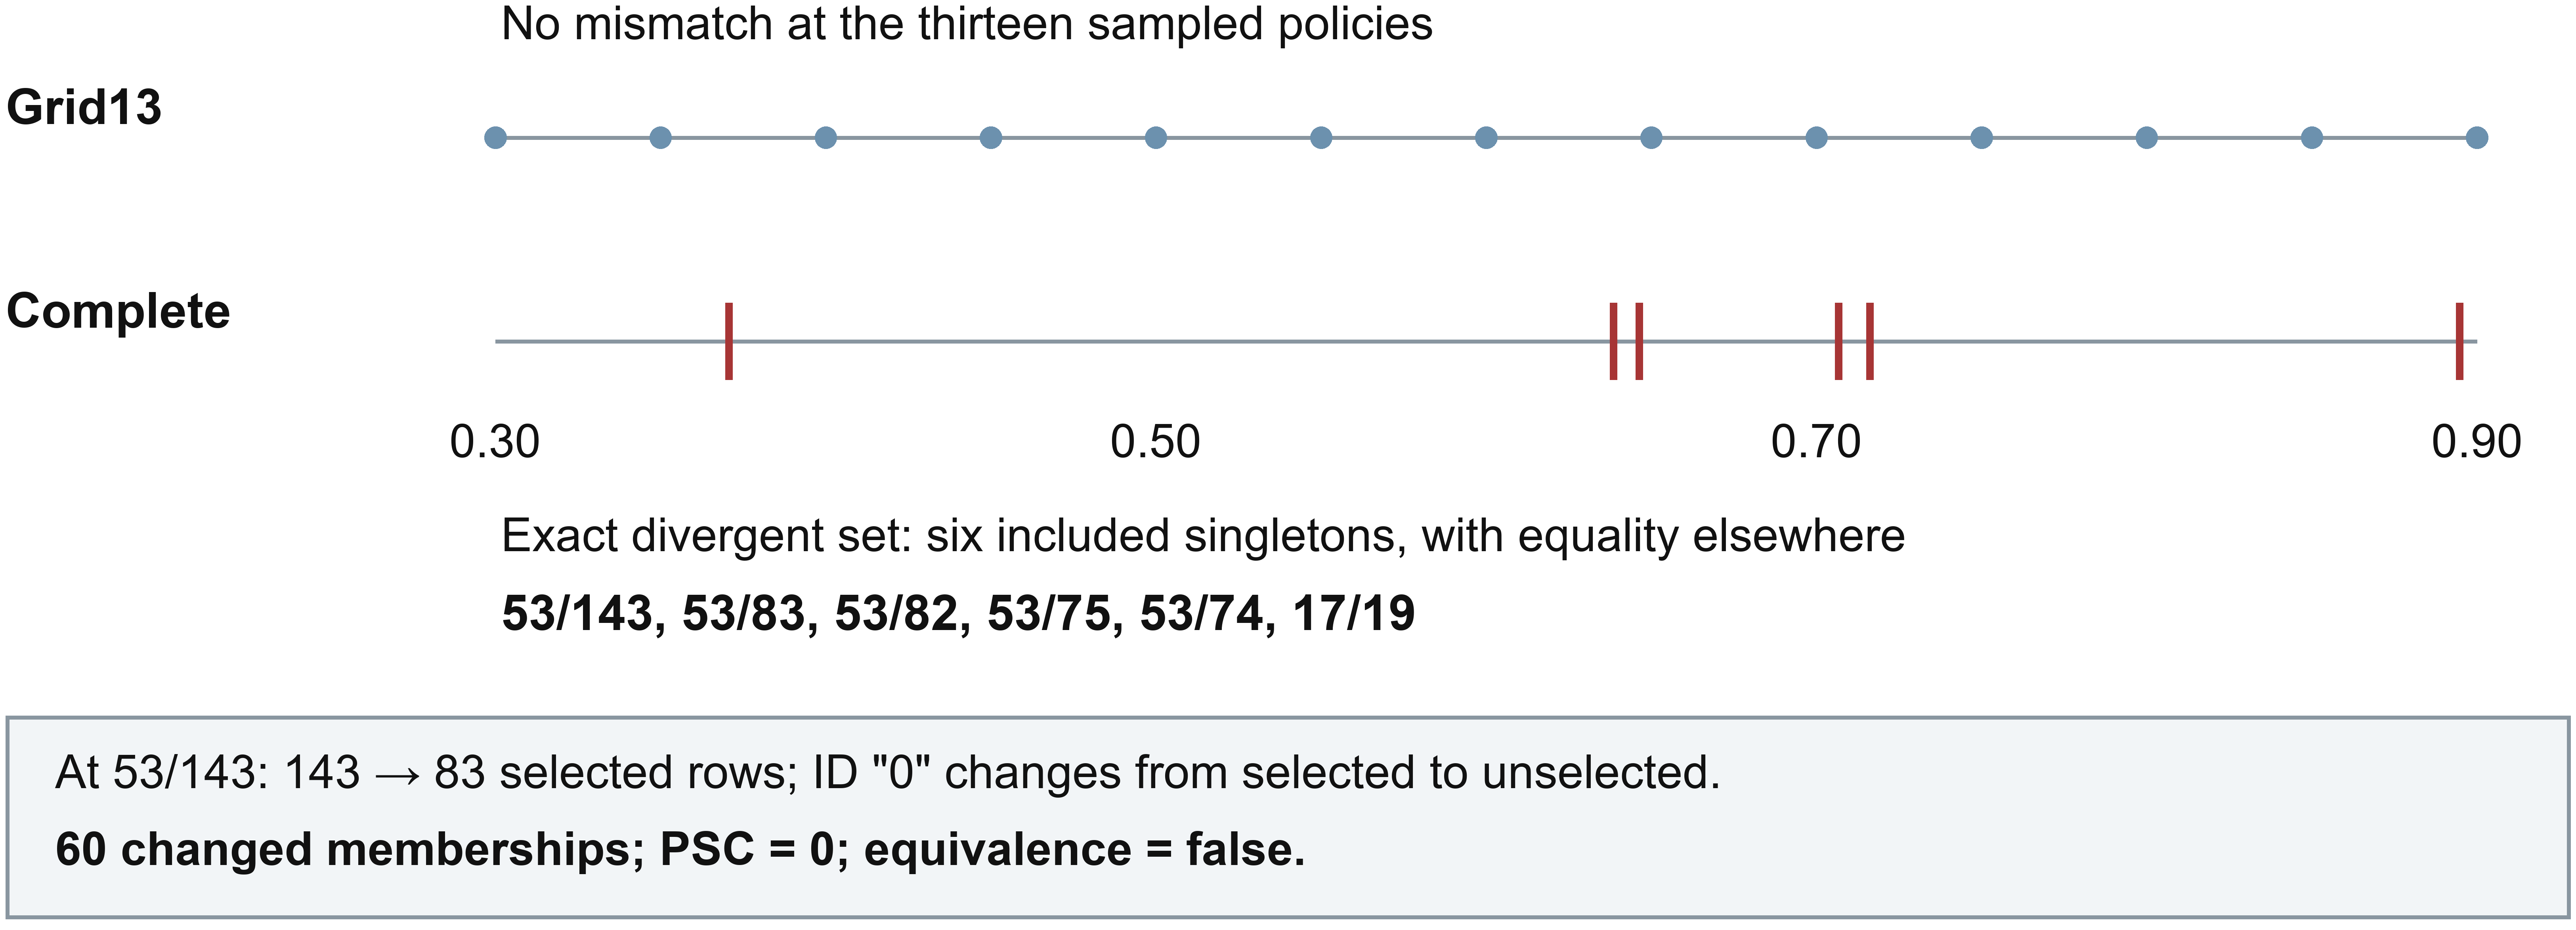
\includegraphics[width=0.88\textwidth]{figures/fig3.png}
\caption{Exact singleton-only regression diagnosis for the strict-precision variant on \texttt{wdbc\_logistic\_isotonic\_seed0}. All six divergent policies are missed by the thirteen-point grid; PSC remains zero despite selected-ID non-equivalence}\label{fig:3}
\end{figure}
\FloatBarrier

The case is bound to \texttt{inputs/\allowbreak case\_068.\allowbreak npz} and \texttt{results/\allowbreak certificates/\allowbreak mutation\_\allowbreak 000.json}. Its mutation CSV row, complete/grid CLI reports and independent direct-mask reconstruction agree on the missed-grid outcome, singleton closure and witness. Online Resource~1 (Section~S21) gives the full locations and hash bindings. The informative result is a complete set with checkable boundary membership, rather than a larger interval-length statistic.

On the two documented upstream defects, grid13 and complete checking identify exactly the same affected workloads: 15 of 31 for scikit-learn and 31 of 36 for SciPy (Table~\ref{tab:7}). Snapshot finds 14 and 26, respectively. Fixed-source and installed-current controls have no policy false alarms. All 108 SciPy affected/fixed/current core certificates are independently replayed using actual interpolation outputs. Complete diagnostics add exact localization, endpoint ownership and replayable membership evidence, but add zero affected-workload detections over grid13 in these cases. The confirmed-defect count remains two; workloads and numerical-interface differentials are not independent bug counts.

\begin{table}[!htbp]
\caption{Detection of affected workloads in the two documented upstream defects; denominator counts describe historical regression fixtures}\label{tab:7}
\centering
\footnotesize
\setlength{\tabcolsep}{3pt}
\renewcommand{\arraystretch}{1.15}
\begin{tabularx}{\textwidth}{@{} >{\raggedright\arraybackslash}X c c c c c @{}}
\toprule
\textbf{Upstream defect} & \textbf{Workloads} & \textbf{Affected} & \textbf{Snapshot} & \textbf{Grid 13} & \textbf{Complete} \\
\midrule
scikit-learn \#23213 & 31 & 15 & 14 & 15 & 15 \\
SciPy \#6318 & 36 & 31 & 26 & 31 & 31 \\
\bottomrule
\end{tabularx}
\end{table}
\FloatBarrier


\subsection{RQ3 Computational and Verification Costs}\label{subsec:rq3}

Complete-region implementations agree on their diagnostic outputs across the 27-task smaller-candidate factorial, with 54 independently replayed certificates and 270 timing records. Partition has the lower total median in 25 of 27 tasks; the remaining two have an equal or smaller SMT median. Table~\ref{tab:8} presents the N=100{,}000 slice. The six larger-candidate tasks produce another 36 timing records and twelve replayed certificates, reaching 430 critical points and 215 components; cases favouring SMT remain in Online Resource~1 (Section~S16).

\begin{table}[!htbp]
\caption{Complete diagnostic comparison at $N = 100{,}000$ over the smaller candidate set ($G \in \{10, 30, 90\}$); five randomized repetitions per condition}\label{tab:8}
\centering
\footnotesize
\setlength{\tabcolsep}{5pt}
\renewcommand{\arraystretch}{1.15}
\begin{tabular}{@{}lrrrr@{}}
\toprule
\textbf{G / omission} & \textbf{Critical points} & \textbf{Components} & \textbf{Partition total ms} & \textbf{SMT total ms} \\
\midrule
10 / alternating & 10 & 5 & 59.26 & 78.39 \\
10 / none & 10 & 0 & 52.90 & 65.71 \\
10 / one & 10 & 1 & 58.68 & 64.17 \\
30 / alternating & 27 & 13 & 111.01 & 193.82 \\
30 / none & 27 & 0 & 100.06 & 109.05 \\
30 / one & 27 & 1 & 103.76 & 129.67 \\
90 / alternating & 79 & 39 & 494.01 & 1058.73 \\
90 / none & 79 & 0 & 323.85 & 317.51 \\
90 / one & 79 & 1 & 329.47 & 391.97 \\
\bottomrule
\end{tabular}
\end{table}
\FloatBarrier

Certificate production and independent checking incur distinct costs. In the traced N=100{,}000 witness-enabled divergent condition, the production median is 528.06 ms (IQR 40.73), with 111 witness-bearing state cells. Its witness-disabled counterpart is 520.59 ms (IQR 120.04); these noisy condition medians do not isolate witness cost by subtraction. The full production and phase records are in Online Resource~1 (Sections~S9--S10 and S16).

On identical prepared certificates, the streaming consumer lowers median checking time in all six paired conditions and substantially reduces retained memory at larger N (Table~\ref{tab:9}). At N=100{,}000 on the divergent fixture, the paired medians are 35,034.92 ms for the materialized checker and 3,557.72 ms for streaming; separately traced peaks are 169.85 and 6.00 MiB (a $28.3\times$ auxiliary memory reduction). This isolates an implementation tradeoff within the consumer obligation. It neither compares against a different producer protocol nor removes the consumer's worst-case counting work. The supporting plot and implementation details are in Online Resource~1 (Section~S17).

\begin{table}[!htbp]
\caption{Paired independent-consumer timing and separately traced auxiliary memory on identical fixtures. Benchmark timings reflect recorded snapshot measurements under Python 3.12.10/NumPy 2.3.5}\label{tab:9}
\centering
\footnotesize
\setlength{\tabcolsep}{5pt}
\renewcommand{\arraystretch}{1.15}
\begin{tabular}{@{}lcccc@{}}
\toprule
\textbf{N / fixture} & \textbf{\makecell{Materialized median\\(IQR), ms}} & \textbf{\makecell{Streaming median\\(IQR), ms}} & \textbf{\makecell{Materialized\\peak MiB}} & \textbf{\makecell{Streaming\\peak MiB}} \\
\midrule
1{,}000 / invariant & 6.41 (0.67) & 2.56 (0.15) & 0.04 & 0.04 \\
1{,}000 / divergent & 26.98 (1.38) & 6.24 (0.46) & 0.09 & 0.04 \\
10{,}000 / invariant & 130.23 (12.14) & 27.72 (6.19) & 1.33 & 0.63 \\
10{,}000 / divergent & 1859.66 (59.43) & 145.62 (22.20) & 3.56 & 0.63 \\
100{,}000 / invariant & 7097.14 (759.47) & 1843.19 (48.92) & 61.42 & 6.00 \\
100{,}000 / divergent & 35034.92 (360.42) & 3557.72 (139.89) & 169.85 & 6.00 \\
\bottomrule
\end{tabular}
\end{table}
\FloatBarrier


\subsubsection{Comparison with Boundary-Aware Direct Probing Baseline}\label{subsubsec:boundary_baseline}

To address whether the certificate-based framework provides an empirical advantage over direct boundary enumeration, Table~\ref{tab:boundary_baseline} evaluates a phase-level comparison between Boundary-Aware Direct Probing and the proposed framework across representative benchmark cohorts under invariant conditions ($N \in \{143, 450, 600, 37{,}471\}$). Both methods operate on identical preprocessed candidate descriptors and evaluate the exact same $2K-1$ critical policy atoms (all $K$ boundary singletons and $K-1$ open-atom midpoints, where $K = |B|$ is the total number of critical boundary values including domain endpoints $L$ and $H$). All timings report medians and interquartile ranges (IQR) across five randomized repetitions under Python 3.11/Windows.

In the core evaluation phase, direct boundary probing scans candidate descriptors across all $2K-1$ probes to select winning thresholds and verify selected bitsets, incurring repeated candidate-scanning costs bounded by $\mathcal{O}((K+C) \cdot G)$. In candidate-dense settings where $G = \Theta(N)$ (the Digits cohort, $N=450, G=450, K=106$), direct probing core takes $75.24\text{ ms}$ (IQR $10.20$), whereas the monotone heap sweep requires only $1.45\text{ ms}$ (IQR $0.20$)---achieving a core algorithmic speedup of $52.0\times$ (and $10.9\times$ on Generated RF). Even when accounting for full certificate assembly, observation witness extraction, and SHA-256 input array hashing, the complete producer median ($3.77\text{ ms}$ on Digits) was below the direct-probing core median ($75.24\text{ ms}$), despite their different output obligations; independent certificate checking is measured separately.

Crucially, the two approaches have different evidential obligations. The evaluated stateless direct probing baseline produces only a transient Boolean verdict, whereas the proposed framework persists an input-bound certificate (independently verifiable against original inputs) that enables streaming consumer verification retaining only a constant number of simultaneously active masks ($11.19\text{ ms}$ on Digits; $24.85\text{ ms}$ on Simulated Cold-Chain). To illustrate the lifecycle impact of these obligations under assumed shared packaging costs, if direct probing were extended to produce the same certificate schema (witness extraction and input hashing, estimated at $2.32\text{ ms}$ on Digits by subtracting sweep core from full producer median) and checked via the same streaming verifier ($11.19\text{ ms}$), the resulting illustrative component-based latency estimate would be $88.75\text{ ms}$ vs. $14.96\text{ ms}$ (an estimated $5.93\times$ end-to-end ratio). We emphasize that this $5.93\times$ figure is an analytical component-based estimate under assumed shared overheads rather than a separately measured paired end-to-end benchmark; the primary measured empirical speedup remains the $52.0\times$ core sweep speedup in Table~\ref{tab:boundary_baseline}. Decomposing the full lifecycle into $T_{\text{total}} = T_{\text{preparation}} + T_{\text{production}} + T_{\text{verification}} + T_{\text{query}}$ illustrates the component-level cost tradeoffs and workload-dependent conditions under which certificate reuse may become advantageous under the evaluated experimental protocols: for the evaluated small WDBC fixture ($N = 143, G = 15$), stateless direct probing had a lower core latency ($0.33\text{ ms}$) than the separate certificate-production ($0.47\text{ ms}$) and verification ($0.76\text{ ms}$) phases. Conversely, when input-bound audit certificates or independent verification are required by the application or its quality-assurance process, the sweep-based architecture provides checkable diagnostic evidence. For repeated sub-domain queries, certificate reuse may amortize setup overhead, depending on workload characteristics and query batch size: once verified, the certificate supports sub-domain interval and point queries in approximately $17\text{--}28\ \mu\text{s}$ ($16.7\text{--}27.7\ \mu\text{s}$ on the four evaluated fixtures in Table~\ref{tab:boundary_baseline}, $\mathcal{O}(\log(M+1))$), whereas the stateless baseline must repeat all $2K-1$ candidate evaluations from scratch. As detailed in the comprehensive reuse evaluation (Online Resource~1 (Sections~S13--S15)), whether certificate reuse yields a net performance advantage depends on query batch size and audit requirements. Finally, while theoretical bounds show asymptotic efficiency, these empirical speedups describe the four evaluated configurations and do not imply universal scaling across all unmeasured $(N, G, K)$ combinations.

\begin{table}[!htbp]
\caption{Phase-level benchmark comparison between Boundary-Aware Direct Probing and the proposed framework across four benchmark cohorts under invariant conditions (five repetitions; median and IQR; Simulated Cold-Chain models $N=37{,}471$ telemetry readings with deterministic rule-based $2\text{--}8^\circ\text{C}$ safe-window excursion criteria)}\label{tab:boundary_baseline}
\centering
\footnotesize
\setlength{\tabcolsep}{3pt}
\renewcommand{\arraystretch}{1.15}
\resizebox{\textwidth}{!}{%
\begin{tabular}{@{}lrrrrrrrr@{}}
\toprule
\textbf{Workload cohort} & \textbf{$N$} & \textbf{$G$} & \textbf{$K$} & \textbf{\makecell{Direct probing\\core ms (IQR)}} & \textbf{\makecell{Sweep producer\\core ms (IQR)}} & \textbf{\makecell{Core\\speedup}} & \textbf{\makecell{Producer full\\cert ms (IQR)}} & \textbf{\makecell{Streaming check\\ms (IQR)}} \\
\midrule
WDBC & 143 & 15 & 8 & 0.33 (0.02) & 0.09 (0.03) & 3.6$\times$ & 0.47 (0.17) & 0.76 (0.10) \\
Digits & 450 & 450 & 106 & 75.24 (10.20) & 1.45 (0.20) & 52.0$\times$ & 3.77 (2.01) & 11.19 (0.80) \\
Generated RF & 600 & 54 & 33 & 3.20 (0.75) & 0.29 (0.02) & 10.9$\times$ & 1.01 (0.01) & 2.25 (0.51) \\
Simulated Cold-Chain & 37{,}471 & 87 & 6 & 0.70 (0.05) & 0.14 (0.01) & 4.8$\times$ & 11.94 (1.14) & 24.85 (1.61) \\
\bottomrule
\end{tabular}%
}
\end{table}
\FloatBarrier


\subsection{RQ4 Policy Domains and Certificate Reuse}\label{subsec:rq4}

The numerical-interface study exposes a difference between continuous-domain diagnosis and membership of a declared query set. Of 30 eval-toolkit workloads, 27 have positive rational-reference PSC and three have zero PSC; the positive median is 3.747190e-16. Exact intersection finds no affected policy on any of the four declared rational decimal lattices. A separate set of 196 representable-binary64 probes exposes differences on 19 workloads. These are different policy embeddings, not contradictory measurements of one query set (Fig.~\ref{fig:4}).

\begin{figure}[!htbp]
\centering
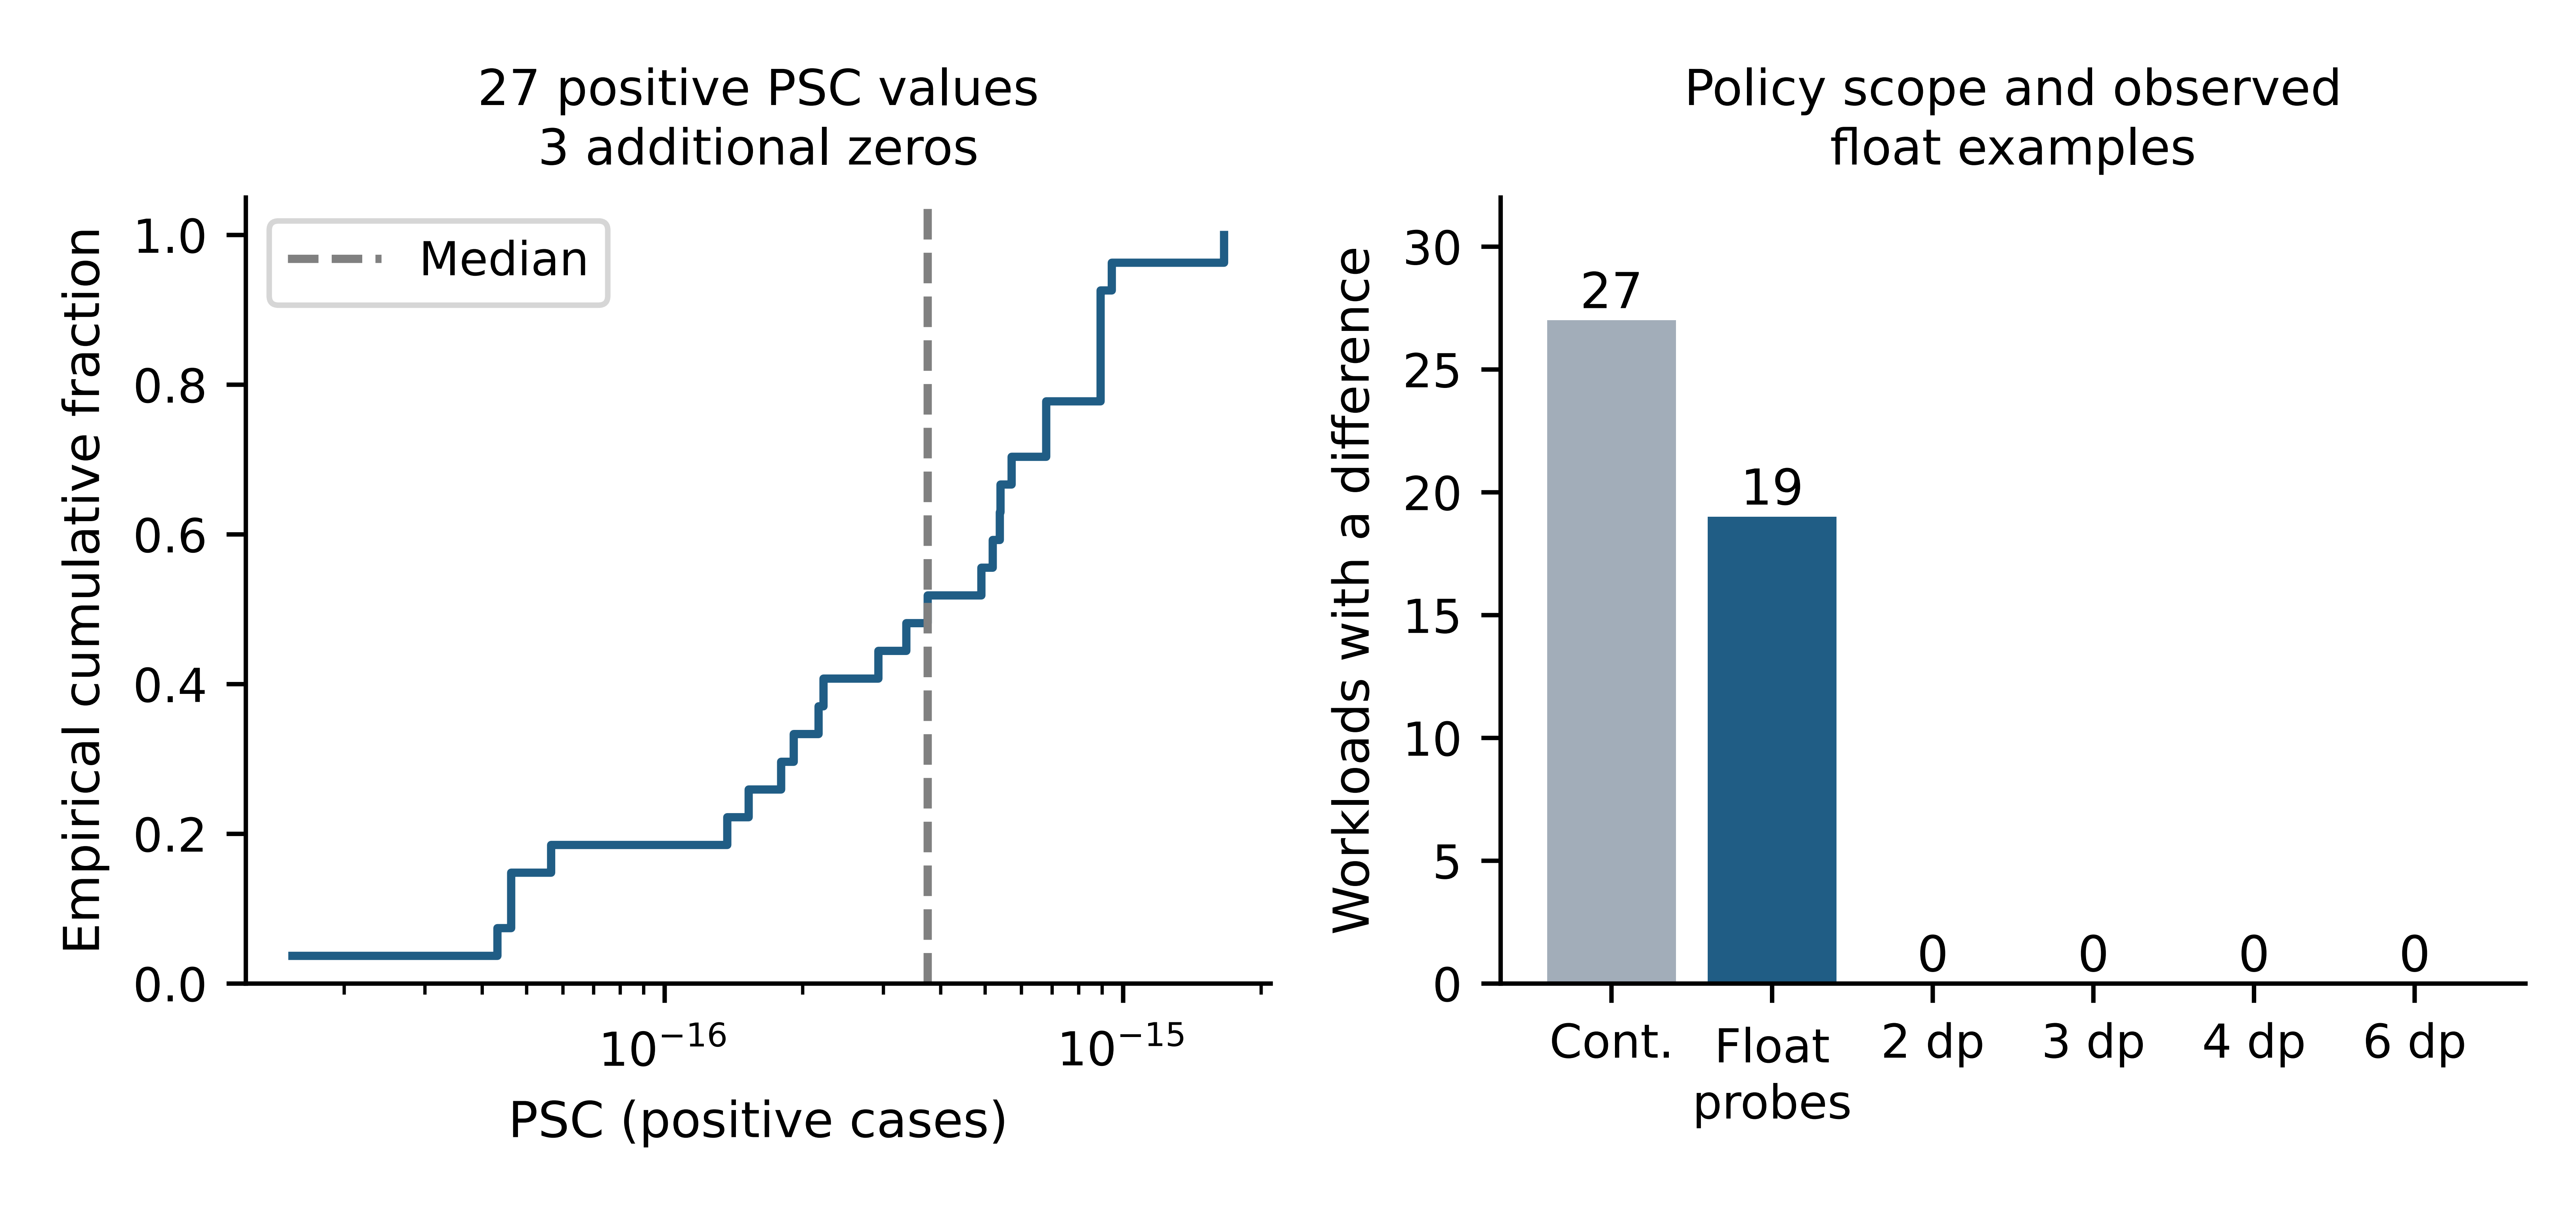
\includegraphics[width=0.88\textwidth]{figures/fig4.png}
\caption{Numerical-interface outcomes under different policy embeddings. Decimal-lattice bars are exact complete intersections; binary64 probes are a separate finite query set. These are not deployment probabilities}\label{fig:4}
\end{figure}
\FloatBarrier

The rational-reference/public-interface guard model agrees with all 884 critical-point/midpoint observations and 1,500 public calls, including baselines. The binary64 probe study compares each representable value by its exact integer ratio, whereas decimal lattices retain exact decimal targets. For illustration, representable float 0.4 exceeds exact 2/5: the five-row $[1, 1, 0, 0, 0]$ ordered-score example selects five versus four at that float's rational embedding, while both select five at exact 2/5. This explains interface semantics; it is separate from the recorded missed-grid case in \S\ref{subsec:rq2} and adds no confirmed library bug. Full distributions, exact intersections and the observed 41-of-64 maximum changed-ID count remain in Online Resource~1 (Section~S8).

On the 36 SciPy fixtures, all 288 allowed-domain query answers agree with independent Z3 checking, with no unknown result. Finite-set and two-/three-place lattice checks cover 24,408 explicit policies; finer lattices use exact intersections. The continuous interval affects 31 workloads, while the declared set {0.50,0.80,0.90} affects 30 (Table~\ref{tab:10}). At two decimal places, 1,611 of 2,196 allowed policy/workload pairs are affected. Those counts describe fixture coverage under declared scenarios, not deployment frequencies.

\begin{table}[!htbp]
\caption{Verified certificate reuse for eight declared policy-domain scenarios on the same 36 workloads}\label{tab:10}
\centering
\footnotesize
\setlength{\tabcolsep}{2.5pt}
\renewcommand{\arraystretch}{1.15}
\begin{tabularx}{\textwidth}{@{} >{\raggedright\arraybackslash}p{4.2cm} >{\centering\arraybackslash}p{2.2cm} >{\centering\arraybackslash}p{2.8cm} >{\centering\arraybackslash}X @{}}
\toprule
\textbf{Allowed policy scenario} & \textbf{\makecell{Policies per\\workload}} & \textbf{\makecell{Workloads with\\affected target}} & \textbf{\makecell{Affected policy/\\workload pairs}} \\
\midrule
Thirteen-point grid & 13 & 31 / 36 & 340 \\
Declared set {0.50,0.80,0.90} & 3 & 30 / 36 & 86 \\
Decimal lattice 2 places & 61 & 31 / 36 & 1,611 \\
Decimal lattice 3 places & 601 & 31 / 36 & 15,886 \\
Decimal lattice 4 places & 6,001 & 31 / 36 & 158,657 \\
Decimal lattice 6 places & 600,001 & 31 / 36 & 15,863,561 \\
Closed interval $[0.30, 0.90]$ & Continuous & 31 / 36 & Not a finite count \\
Closed interval [0.80,0.90] & Continuous & 30 / 36 & Not a finite count \\
\bottomrule
\end{tabularx}
\end{table}
\FloatBarrier

Certificate reuse changes costs without changing that diagnostic contract. The paired API study retains 960 timing records, 192 groups and 40,560 agreeing repeated method answers over 2,028 existing query plans. At batch 128, the Boolean API lowers query-phase medians in all twelve paired combinations, but lowers total medians, including setup and full checking, in eleven. Against direct masks it has lower totals in 2/6 point and 6/6 window cases under unequal certificate obligations. Thus query-phase speedups do not establish an end-to-end break-even guarantee. Detailed route obligations, total-cost tables and all batches are in Online Resource~1 (Sections~S13--S15 and S17).


\section{Discussion}\label{sec:discussion}


\subsection{Interpretation of the Main Findings}

The central finding is that policy-wide selected-ID diagnosis requires explicit coverage and ownership information that point observations and interval length do not supply by themselves. The recorded WDBC strict-feasibility case makes this distinction concrete: grid13 sees agreement, PSC is zero, yet six admitted policy values change membership. The result follows from the contract and exact boundary semantics, with an observation-level witness available for replay.

The upstream studies answer a different question. Because grid13 detects every affected workload in both documented cases, they establish applicability and diagnostic scope rather than an external detection advantage. A certificate adds the complete location of the change and binds it to inputs and memberships that another implementation can check. That is a technical basis for inspection and handoff.


\subsection{Analytical Insights and Practical Adoption Boundaries}\label{subsec:discussion_insights}

Analyzing why 57 of the 240 valid selector/numerical fault variants (23.75\%) exhibit exact policy equivalence despite code modifications reveals a key property of precision-constrained selectors: candidate redundancy. One mechanism that can explain such equivalence is that when a mutation modifies a candidate threshold whose precision-recall profile is strictly Pareto-dominated across the entire domain $[L, H]$, or perturbs feasibility guards outside the achievable score range, the upper envelope of winning thresholds remains unchanged. Consequently, neither observation memberships nor boundary ownerships diverge. Complete diagnosis formally verifies this equivalence, avoiding false-alarm refactoring in continuous regression pipelines.

The empirical results also delineate when grid sampling is practically sufficient versus when complete certification is necessary. For routine continuous-integration triage where operating thresholds are empirically known to remain safely distant from critical ratios under specific workload assumptions, grid sampling may provide fast, lightweight feedback; this observation, however, remains strictly conditional on threshold placement rather than a universal guarantee for arbitrary CI pipelines. However, in high-stakes auditing, safety-critical decision systems, or when operating conditions span exact boundary singletons, grid sampling fails ($PSC=0$ while dozens of observation decisions swap, as shown in Fig.~\ref{fig:3}). In such settings, an input-bound certificate may provide valuable independently checkable diagnostic evidence when persistent auditability is an explicit application requirement.

Regarding the cost-benefit trade-off, complete certification may become advantageous for some repeated-query workloads when setup costs are sufficiently amortized ($\approx 17\text{--}28\ \mu\text{s}$ per query vs. repeated full-dataset evaluation), or when independently checkable diagnostic evidence is required. Conversely, for the evaluated small WDBC fixture ($N = 143, G = 15$), stateless direct probing achieved lower core latency ($0.33\text{ ms}$) than the separate certificate-production ($0.47\text{ ms}$) and verification ($0.76\text{ ms}$) phases.

Deploying this framework in broader software systems requires recognizing its core technical constraints. The reduction to finite critical cuts applies generally to finite-candidate selectors with deterministic numerical mappings (such as IEEE 754 float32/float64 rounding cuts). The most challenging requirement in practice is maintaining aligned observation IDs across versions. If a refactoring dynamically alters how candidate families are generated per policy target or perturbs observation ordering, the framework cannot establish selected-ID equivalence and must safely refuse certification. Refusal is an intentional design boundary ensuring that unverified assumptions are never silently certified. Related classifier testing \cite{duquetorres2025assessing,yang2021towards,xie2011testing}, robust classification \cite{provost2001robust} and parametric monitoring \cite{chen2009parametric} address different observables, as detailed in Online Resource~1 (Section~S24).


\subsection{Implications for Regression Diagnosis and Release Assurance}

A release requirement should declare observation identities, selector semantics, numerical conversion and the policies to preserve. A diagnostic result can then distinguish checked equivalence, an exact affected region with a witness, and refusal because assumptions are unsupported. An affected singleton must not be erased by a numerical tolerance or hidden by zero PSC. Conversely, a rational-reference difference does not become an upstream defect unless that contract is actually required.

Whether retaining a certificate is worthwhile depends on the need for persistent, independently checkable scope and on construction, checking, storage and query costs. Streaming reduces one consumer's retained masks, and the Boolean index avoids unnecessary intersection output; both preserve setup obligations. A small fixed policy set can favour direct masks. Broader adoption benefits in human-in-the-loop settings are open for prospective evaluation.


\subsection{Threats to Validity and Limitations}

Internal and construct validity depend on a shared mathematical contract, correctly represented guard changes and faithful adapters. Separately coded consumers can share conceptual errors, and finite tests are not machine-checked proofs. Input hashes bind bytes, not dataset authenticity or label quality. In particular, AST restrictions and consistent sampled guard events cannot certify arbitrary stateful Python programs; refusal is part of the admitted method.

External validity is limited by related stored comparisons, three local pipeline families, hand-designed variants and two historical-source defect replays with compatibility bridges. The pharmaceutical cold-chain telemetry scenario represents a simulated monitoring application under deterministic rule-based criteria ($2\text{--}8^\circ\text{C}$), not an empirical validation on an operational, deployed enterprise alert system. The condition-coverage table shows which assumptions are challenged, not a representative distribution of deployed systems. Multiple random seeds and constructed propagation fixtures challenge numerical sensitivity but do not represent independent industrial software deployments or new in-the-wild bug distributions. Furthermore, full execution is recorded on a verified Windows host. Frozen input arrays and deterministic byte hashes support input integrity and cross-environment result comparison, but do not by themselves guarantee numerical reproducibility across platforms. Native cross-platform execution (e.g., containerized Linux CI pipelines) and independent prospective developer studies remain open avenues for external validation.

Performance validity is restricted to recorded hosts, input structures, repetition counts and instrumentation. Traced and untraced protocols, producer and consumer work, and equal versus unequal certificate obligations remain separate. Arbitrary-precision operands and $\mathcal{O}(NG)$/$\mathcal{O}(ND)$ checking or witness work can dominate.


\section{Conclusion}\label{sec:conclusion}

Selected-ID equivalence across a permitted policy domain is conditionally reducible to finitely many exact membership checks when candidate identities, fixed priorities and every numerical guard cut are represented. Retaining singleton ownership and checking an input-bound certificate preserve information that sampled agreement and divergent interval length can lose. The recorded six-singleton case demonstrates that distinction on an evaluated input.

Controlled studies support the implemented diagnostic obligations and expose missed point coverage; two documented upstream defects support applicability and exact localization with no additional affected-workload detection over grid13. Engineering studies quantify the costs of obtaining and reusing checkable diagnostics. The result is an evaluated specification for this finite selector contract; extending its assurance scope to broader program classes and independent deployments is a natural next step.


\section{Reproducibility and Data Availability}

The submission package provides the research artifact and detached execution report as Online Resources~2 and~3 alongside the manuscript and Supplementary Material (Online Resource~1). The exact artifact SHA-256 is \texttt{\seqsplit{98cfc7ec8498214a79717480e5a8be83707cc4244296fe3cb589a329dc4fa8aa}}. It supplies frozen inputs, source, tests, measurements, certificates, dependency specifications and the eval-toolkit wheel; it is not a complete bundled Python environment. Source, dependency and dataset licenses accompany their respective materials. Full repository and archiving details are listed under Statements and Declarations.

After extraction and dependency installation under the recorded Python 3.13.18 environment, the single computational entry point is python run\_all.py from the artifact root. The detached report records 33 successful stages in 2,345.58 seconds on Windows, including 42 core tests and 18 separate upstream tests. This is a recorded duration, not a runtime bound. Frozen-input reproduction is the default; historical dependency-binary re-execution and optional model retraining have additional requirements and distinct assurance scopes. Online Resource~1 (Section~S21) gives installation commands, environment versions, expected outcomes, manifest identities and the result-to-file map.

The reading copy uses recorded benchmark snapshots. Regenerated execution timings retain their own records, and not every output is byte-identical. The Evidence package distributes all changed/new output bytes with a field-level reconciler; it separates record verification from independent computational execution. Historical manuscript-generation stages can regenerate earlier editorial layouts, so the current submission manuscript is supplied separately. No new full-pipeline execution is claimed for this document revision.


\section*{Supplementary Information}
Supplementary material accompanies this article as Online Resource~1 (ESM\_1.pdf) and provides complete formal diagnostic specifications and proofs (Part A, Section~S1), extended empirical validity studies on fresh dependencies, program conformance, mutation records, upstream replays, and numerical interface lattices (Part B, Sections~S2--S8), engineering feasibility benchmarks, algorithmic cost decompositions, SMT comparison baselines, and streaming memory profiles (Part C, Sections~S9--S17), reproducibility manifests and artifact verification protocols (Part D, Sections~S18--S21), and detailed mappings to foundational verification literature (Part E, Sections~S22--S24). All citations match the numbered bibliography [1]--[29].

\section*{Acknowledgements}
Generative AI tools (OpenAI Codex) were used to assist with manuscript organization, language revision, mathematical presentation, authoring scripts, baseline adapters and execution harnesses. The associated research artifact contains assistant-generated code and prose. All scientific claims, formal proofs, experimental evaluations, code outputs, and final texts were reviewed and approved by the authors, who take full responsibility for the contents of this publication.

\section*{Declarations}
\subsection*{Funding}
This research was supported by the University of Economics Ho Chi Minh City (UEH), Vietnam. No external grants or commercial funds were received for this study.

\subsection*{Competing interests}
The authors declare no competing financial or non-financial interests.

\subsection*{Ethics approval and consent to participate}
Not applicable. This study does not involve human participants, animal subjects, or sensitive personal data.

\subsection*{Consent for publication}
Not applicable.

\subsection*{Data availability}
The evaluation data and benchmark records are provided in Online Resource~2 (\texttt{Reproduci\allowbreak bility\_\allowbreak Artifact.\allowbreak zip}, SHA-256: \texttt{\seqsplit{98cfc7ec8498214a79717480e5a8be83707cc4244296fe3cb589a329dc4fa8aa}}) and will be archived on Zenodo upon acceptance. Public evaluation data include the Wisconsin Diagnostic Breast Cancer (WDBC) dataset (UCI Machine Learning Repository, DOI:\allowbreak\ \url{https://doi.org/10.24432/C5DW2B}).

\subsection*{Materials availability}
Not applicable.

\subsection*{Code availability}
All source code, oracle checkers, streaming consumers, and benchmark evaluation scripts are distributed in Online Resource~2. Detached execution logs and field-level verification reconciliations are provided in Online Resource~3 (\texttt{Reproducibility\_\allowbreak Evidence.\allowbreak zip}, SHA-256: \texttt{\seqsplit{0e30a95b24d08cde64e68778d0eba1e211af97e68fe950ff76f021a22793115b}}).

\subsection*{Author contributions}

Conceptualization, B.T.H. and B.H.N.;
methodology, B.T.H. and T.D.K.T.;
software, B.T.H., T.D.K.T. and T.M.N.;
validation, B.T.H., T.D.K.T., B.H.N. and T.M.N.;
formal analysis, B.T.H.;
investigation, B.T.H., T.D.K.T., B.H.N. and G.H.T.;
data curation, T.D.K.T. and T.M.N.;
visualization, B.T.H., B.H.N. and G.H.T.;
writing--original draft preparation, B.T.H., B.H.N. and G.H.T.;
writing--review and editing, T.B.N., B.T.H., T.D.K.T., T.M.N. and G.H.T.;
supervision, T.B.N.;
project administration, T.B.N.

All authors have read and approved the final version of the manuscript.

\begin{thebibliography}{29}
\bibitem{rath2022optimizing}
Rath, P., Hughes, M.: Optimizing early warning classifiers to control false alarms via a minimum precision constraint. PMLR \textbf{151}, 4895--4914 (2022). \url{https://proceedings.mlr.press/v151/rath22a.html}

\bibitem{mackey2018constrained}
Mackey, A., Luo, X., Eban, E.: Constrained classification and ranking via quantiles (2018). \url{https://arxiv.org/abs/1803.00067}

\bibitem{tasche2018plugin}
Tasche, D.: A plug-in approach to maximising precision at the top and recall at the top (2018). \url{https://arxiv.org/abs/1804.03077}

\bibitem{duquetorres2025assessing}
Duque-Torres, A., Klammer, C., Fischer, S., Pfahl, D., Ramler, R.: Assessing the strength of metamorphic testing applied to optimisation software---experience from industry. Inf. Softw. Technol. \textbf{186}, 107807 (2025). \url{https://doi.org/10.1016/j.infsof.2025.107807}

\bibitem{sklearn_calibrated}
scikit-learn developers: CalibratedClassifierCV, version 1.9.1 documentation (2026). \url{https://scikit-learn.org/stable/modules/generated/sklearn.calibration.CalibratedClassifierCV.html}. Accessed 30 Oct 2026

\bibitem{storm2026parametric}
Storm project: Running Storm on parametric models. Official documentation (2026). \url{https://www.stormchecker.org/documentation/usage/running-storm-on-parametric-models}. Accessed 30 Oct 2026

\bibitem{junges2024parameter}
Junges, S., \'{A}brah\'{a}m, E., Hensel, C., Jansen, N., Katoen, J.-P., Quatmann, T., Volk, M.: Parameter synthesis for Markov models: covering the parameter space. Form. Methods Syst. Des. \textbf{62}, 181--259 (2024). \url{https://doi.org/10.1007/s10703-023-00442-x}

\bibitem{godlin2009regression}
Godlin, B., Strichman, O.: Regression verification. In: 46th Annual Design Automation Conference (DAC), pp. 466--471 (2009). \url{https://ofers.dds.technion.ac.il/publications/dac09.pdf}

\bibitem{alkassar2013framework}
Alkassar, E., B\"{o}hme, S., Mehlhorn, K., Rizkallah, C.: A framework for the verification of certifying computations (2013). \url{https://arxiv.org/abs/1301.7462}

\bibitem{necula2002proof}
Necula, G.C., Schneck, R.R.: Proof-carrying code with untrusted proof rules. In: International Symposium on Software Security (ISSS) (2002). \url{https://people.eecs.berkeley.edu/~necula/ISSS02/}

\bibitem{yang2021towards}
Yang, Y., Li, Z., Wang, H., Xu, C., Ma, X.: Towards effective metamorphic testing by algorithm stability for linear classification programs. J. Syst. Softw. \textbf{180}, 111012 (2021). \url{https://doi.org/10.1016/j.jss.2021.111012}

\bibitem{xie2011testing}
Xie, X., Ho, J.W.K., Murphy, C., Kaiser, G., Xu, B., Chen, T.Y.: Testing and validating machine learning classifiers by metamorphic testing. J. Syst. Softw. \textbf{84}(4), 544--558 (2011). \url{https://doi.org/10.1016/j.jss.2010.11.920}

\bibitem{scipy_news}
SciPy project: Release news and versions 1.15.3 and 1.18.1 (2026). \url{https://scipy.org/news/}

\bibitem{sklearn_issue23213}
scikit-learn issue \#23213: precision\_recall\_curve is not returning the full curve at high recall. Upstream bug report and maintainer discussion (2022). \url{https://github.com/scikit-learn/scikit-learn/issues/23213}

\bibitem{sklearn_pr23214}
scikit-learn PR \#23214: FIX compute precision-recall at 100\% recall. Merged 2 May 2022 (2022). \url{https://github.com/scikit-learn/scikit-learn/pull/23214}

\bibitem{demoura2008z3}
de Moura, L., Bj{\o}rner, N.: Z3: an efficient SMT solver. In: Tools and Algorithms for the Construction and Analysis of Systems (TACAS). LNCS, vol. 4963, pp. 337--340. Springer, Heidelberg (2008). \url{https://www.microsoft.com/en-us/research/publication/z3-an-efficient-smt-solver/}

\bibitem{mcconnell2011certifying}
McConnell, R.M., Mehlhorn, K., N\"{a}her, S., Schweitzer, P.: Certifying algorithms. Comput. Sci. Rev. \textbf{5}(2), 119--161 (2011). \url{https://doi.org/10.1016/j.cosrev.2010.09.009}

\bibitem{provost2001robust}
Provost, F., Fawcett, T.: Robust classification for imprecise environments. Mach. Learn. \textbf{42}, 203--231 (2001). \url{https://arxiv.org/abs/cs/0009007}

\bibitem{chen2009parametric}
Chen, F., Ro\c{s}u, G.: Parametric trace slicing and monitoring. In: Tools and Algorithms for the Construction and Analysis of Systems (TACAS). LNCS, vol. 5505, pp. 246--261. Springer, Heidelberg (2009). \url{https://experts.illinois.edu/en/publications/parametric-trace-slicing-and-monitoring/}

\bibitem{dehnert2015prophesy}
Dehnert, C., Junges, S., Jansen, N., Corzilius, F., Volk, M., Bruintjes, H., Katoen, J.-P., \'{A}brah\'{a}m, E.: PROPhESY: A PRObabilistic ParamEter SYnthesis Tool. In: Computer Aided Verification (CAV). LNCS, vol. 9206, pp. 214--231. Springer, Cham (2015). \url{https://www.cs.ru.nl/personal/nilsjansen/files/publications/dehnert-et-al-cav-2015.pdf}

\bibitem{sklearn_tuned}
scikit-learn developers: TunedThresholdClassifierCV, version 1.9.1 documentation: callable scorer, explicit threshold arrays and prefit configuration (2026). \url{https://scikit-learn.org/stable/modules/generated/sklearn.model_selection.TunedThresholdClassifierCV.html}. Accessed 30 Oct 2026

\bibitem{behring2026evaltoolkit}
Behring, B.: eval-toolkit: threshold selection methodology and source (2026). \url{https://brandon-behring.github.io/eval-toolkit/methodology/thresholds.html}. Pinned packaging/source at \url{https://github.com/brandon-behring/eval-toolkit/tree/a6400e74c4534d6d79f17dee11ad903b6d664980}. Accessed 30 Oct 2026

\bibitem{mathsat_api}
MathSAT developers: API reference: msat\_all\_sat, enumeration over important atoms (2026). \url{https://mathsat.fbk.eu/apireference.html}. Accessed 30 Oct 2026

\bibitem{morettin2017efficient}
Morettin, P., Passerini, A., Sebastiani, R.: Efficient weighted model integration via SMT-based predicate abstraction. In: Proceedings of the 26th International Joint Conference on Artificial Intelligence (IJCAI), pp. 720--728 (2017). \url{https://doi.org/10.24963/ijcai.2017/100}

\bibitem{spallitta2025disjoint}
Spallitta, G., Sebastiani, R., Biere, A.: Disjoint projected enumeration for SAT and SMT without blocking clauses. Artif. Intell. \textbf{345}, 104346 (2025). \url{https://doi.org/10.1016/j.artint.2025.104346}

\bibitem{andrlon2023finding}
Andrlon, M.: Finding normal binary floating-point factors efficiently. J. Autom. Reason. \textbf{67}(1), 11 (2023). \url{https://doi.org/10.1007/s10817-023-09660-w}

\bibitem{scipy_issue6318}
SciPy issue \#6318: Scipy interp1d nearest not working for high values on x-axis. Upstream defect report (2016). \url{https://github.com/scipy/scipy/issues/6318}

\bibitem{scipy_pr6351}
SciPy PR \#6351: BUG: \#6318 Interp1d nearest integer x-axis overflow issue fixed. Merged 6 July 2016 (2016). \url{https://github.com/scipy/scipy/pull/6351}

\bibitem{ieee2019floating}
IEEE: IEEE Standard for Floating-Point Arithmetic. IEEE Std 754-2019, pp. 1--84 (2019). \url{https://doi.org/10.1109/IEEESTD.2019.8766229}
\end{thebibliography}

\end{document}
